\documentclass{article}
\usepackage[UTF8]{ctex}
\usepackage{graphicx}
\usepackage[top=3cm, bottom=2cm, left=2.5cm, right=2.5cm]{geometry}
\usepackage[colorlinks=true, allcolors=blue]{hyperref}
\usepackage{float}


\title{实验报告2}
\author{伍紫涵}
\begin{document}
\renewcommand{\maketitle}{
    \begin{titlepage}
        \centering
        {\Huge\bfseries 实验报告2 \par}
        \vspace{2cm}
        
\includegraphics[width=0.7\linewidth]{ouc.png} \par
        \vspace{2cm}
        {\LARGE 姓名:伍紫涵 \par}
        \vspace{1cm}
        {\LARGE 专业:计算机科学与技术 \par}
        \vspace{1cm}
        {\large \today \par}
    \end{titlepage}
}
\maketitle
\begin{titlepage}
\begin{abstract}
本文是我学习的关于shell和vim的实验报告,接下来我会详细地介绍我学习的内容,本文的LaTeX代码已经上传到了\href{https://github.com/qiqiqisi/Latex_Used.git}{github仓库}中,可以点击超链接进行查看。
\end{abstract}
{\hypersetup{hidelinks}\tableofcontents}
\end{titlepage}
\section{shell指令的学习}
\subsection{ls}
ls可以用于查看当前目录的内容。
\begin{figure}[H]
    \centering
    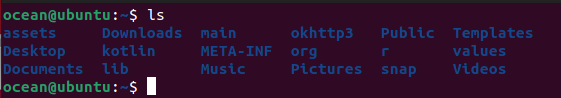
\includegraphics[width=1\linewidth]{ls.png}
\end{figure}

\subsection{cd ..}
cd ..返回当前目录的上一级父目录。
\begin{figure}[H]
    \centering
    
\includegraphics[width=1\linewidth]{cd1.png}
\end{figure}

\subsection{cd <name>}
cd <name>用于进入当前目录中的name层,同样也是更换当前目录。
\begin{figure}[H]
    \centering
    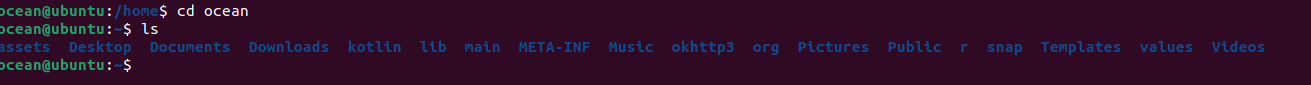
\includegraphics[width=1\linewidth]{cd2.png}
\end{figure}

\subsection{pwd}
pwd用于显示当前工作目录的完整路径。
\begin{figure}[H]
    \centering
    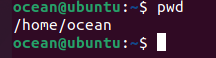
\includegraphics[width=1\linewidth]{pwd.png}
\end{figure}

\subsection{mkdir}
mkdir用于在当前目录创建应该文件夹。
\begin{figure}[H]
    \centering
    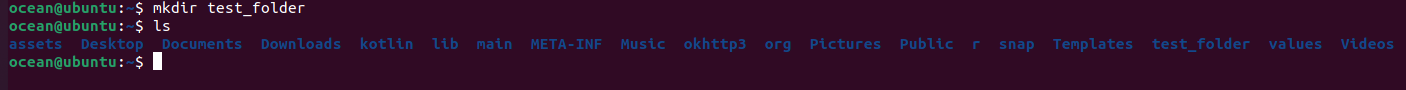
\includegraphics[width=1\linewidth]{mkdir.png}
\end{figure}
\begin{figure}[H]
    \centering
    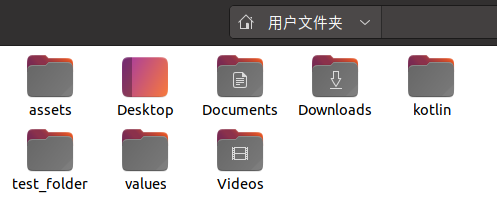
\includegraphics[width=1\linewidth]{folder.png}
\end{figure}

\subsection{rmdir}
rmdir用于删除空文件夹。
\begin{figure}[H]
    \centering
    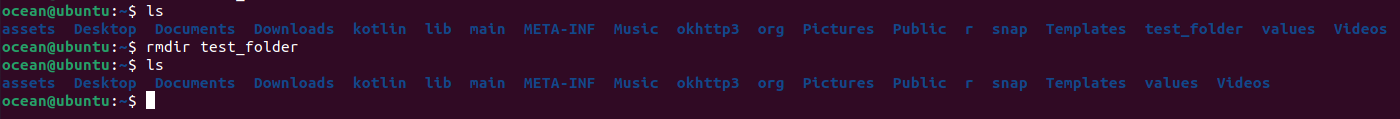
\includegraphics[width=1\linewidth]{rmdir.png}
\end{figure}

\subsection{rm}
rm用于删除文件或者目录。
\begin{figure}[H]
    \centering
    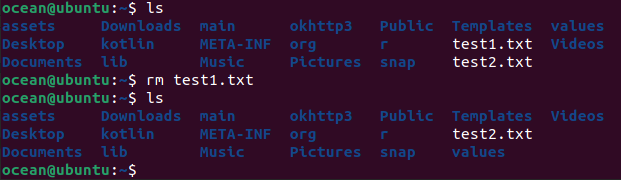
\includegraphics[width=1\linewidth]{rm.png}
\end{figure}

\subsection{mv}
mv <old\_name> <new\_name>用于修改文件名。
\begin{figure}[H]
    \centering
    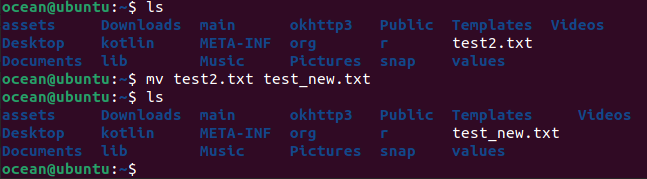
\includegraphics[width=1\linewidth]{mv.png}
\end{figure}

\subsection{赋值并打印操作}
""表示打印这个变量的值。
\begin{figure}[H]
    \centering
    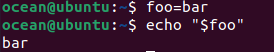
\includegraphics[width=1\linewidth]{print_value.png}
\end{figure}

\subsection{打印字符串而非赋值}
''表示作为字符串直接打印出来。
\begin{figure}[H]
    \centering
    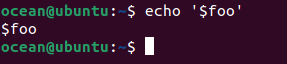
\includegraphics[width=1\linewidth]{print_string.png}
\end{figure}

\subsection{自定义函数}
自定义函数中,\$1代表函数输入的参数。
\begin{figure}[H]
    \centering
    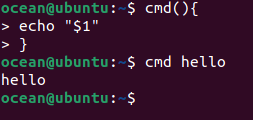
\includegraphics[width=1\linewidth]{function.png}
\end{figure}

\subsection{||}
从左往右,如果第一个是错误的,就执行第二个,如果第一个是正确的,就不执行第二个。
\begin{figure}[H]
    \centering
    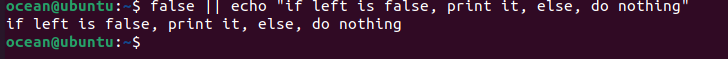
\includegraphics[width=1\linewidth]{or.png}
\end{figure}

\subsection{\&\&}
从左往右,如果第一个是正确的,就执行第二个,如果第一个是错误的,就不执行第二个。
\begin{figure}[H]
    \centering
    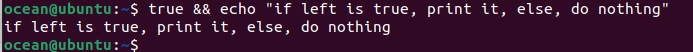
\includegraphics[width=1\linewidth]{and.png}
\end{figure}

\subsection{;}
从左往右依次做这件事。
\begin{figure}
    \centering
    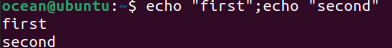
\includegraphics[width=1\linewidth]{both.png}
\end{figure}

\section{Vim}
\subsection{vim <name>}
vim <name>用于打开一个文件,如果这个文件在当前目录下不存在,那么就创建一个这个文件。
\begin{figure}[H]
    \centering
    
\includegraphics[width=1\linewidth]{vim.png}
\end{figure}

\subsection{i}
i切换为代表插入模式。如果在其他模式中,需要在此之前要按下Esc切换到正常模式。
\begin{figure}[H]
    \centering
    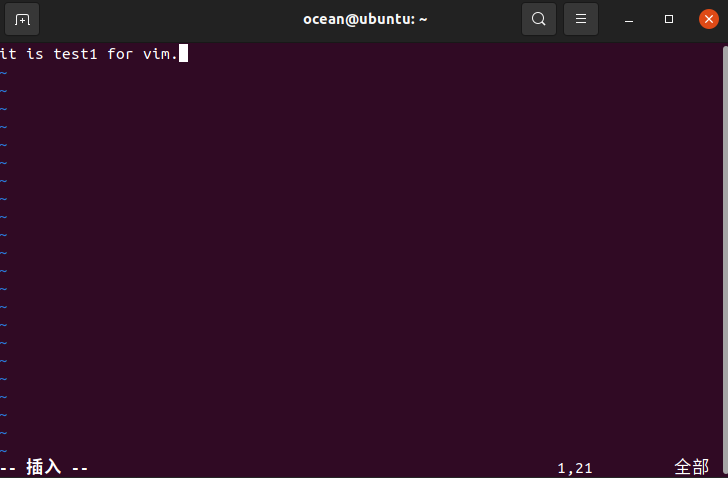
\includegraphics[width=1\linewidth]{insert.png}
\end{figure}

\subsection{:w}
:w代表保存文本。如果在其他模式中,需要在此之前要按下Esc切换到正常模式。
\begin{figure}[H]
    \centering
    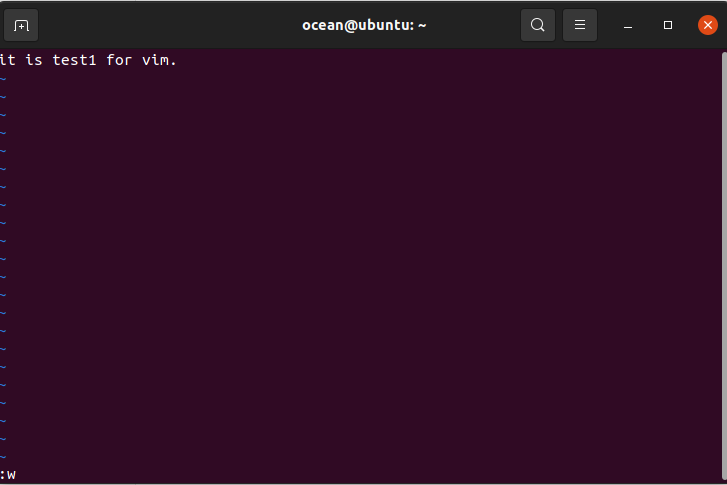
\includegraphics[width=1\linewidth]{w.png}
\end{figure}
\begin{figure}[H]
    \centering
    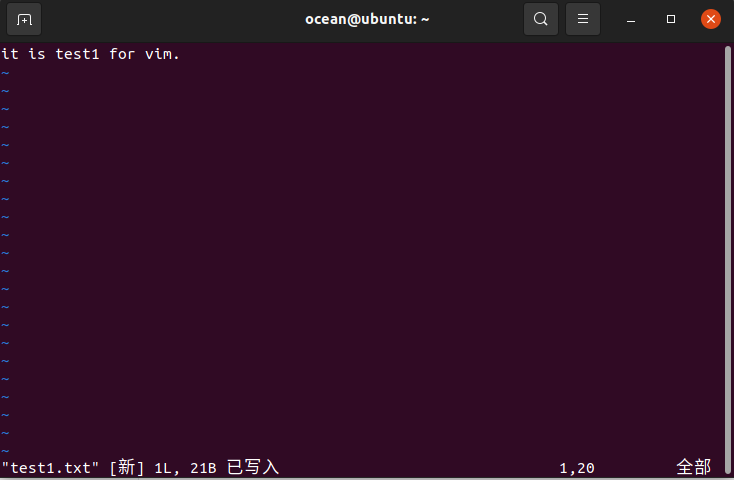
\includegraphics[width=1\linewidth]{w2.png}
\end{figure}

\subsection{:wq}
:wq代表保存并退出。如果在其他模式中,需要在此之前要按下Esc切换到正常模式。
\begin{figure}[H]
    \centering
    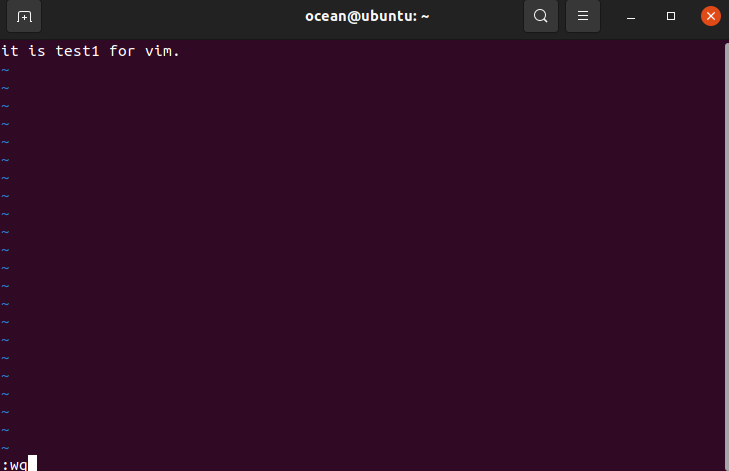
\includegraphics[width=1\linewidth]{wq.png}
\end{figure}

\subsection{:e <name>}
:e <name>代表切换到其他文件。如果在其他模式中,需要在此之前要按下Esc切换到正常模式。
\begin{figure}[H]
    \centering
    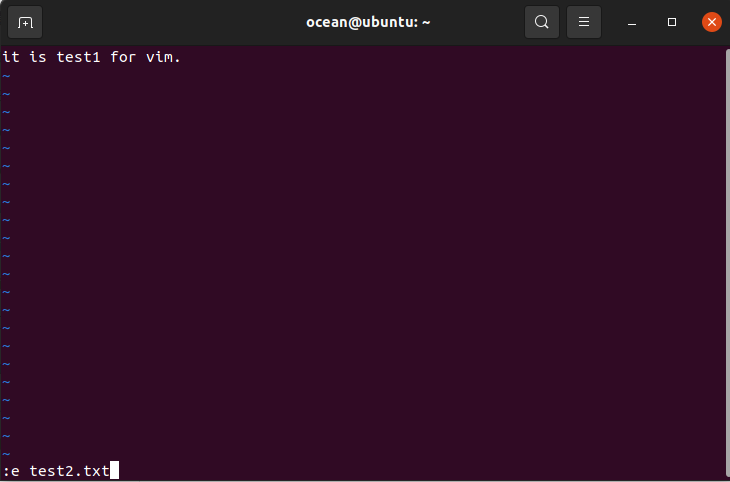
\includegraphics[width=1\linewidth]{e1.png}
\end{figure}

\begin{figure}[H]
    \centering
    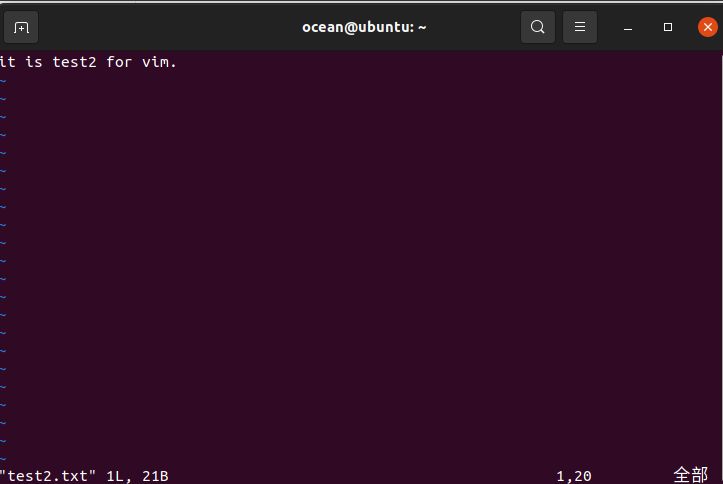
\includegraphics[width=1\linewidth]{e2.png}
\end{figure}

\subsection{:ls}
:ls示打开的缓存。如果在其他模式中,需要在此之前要按下Esc切换到正常模式。
\begin{figure}[H]
    \centering
    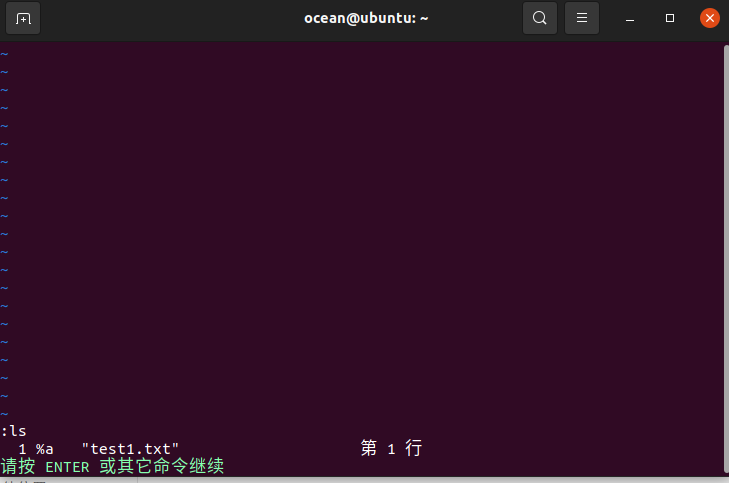
\includegraphics[width=1\linewidth]{ls_tool.png}
\end{figure}

\subsection{3w}
在正常模式下输入3w可以让光标定位到当前光标后的第三个单词。
\begin{figure}[H]
    \centering
    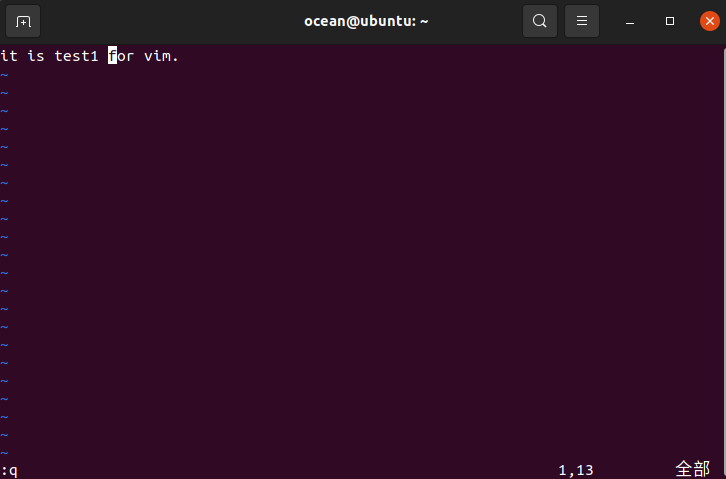
\includegraphics[width=1\linewidth]{3w.png}
\end{figure}
\end{document}
